\documentclass[letterpaper]{article}
\usepackage{natbib,alifexi}
\usepackage[utf8x]{inputenc}

\usepackage{xcolor}

\title{Plan-Based Reward Shaping for Multi-Agent Reinforcement Learning}
\author{Jérôme Bastogne$^{1}$, Maxime Desclefs$^{1}$ \and Simon Picard$^{1}$ \\
\mbox{}\\
$^1$Université Libre de Bruxelles, Boulevard du Triomphe - CP 212, 1050 Brussels, Belgium \\
jbastogn@ulb.ac.be, mdesclef@ulb.ac.be, spicard@ulb.ac.be}


\begin{document}
\maketitle

\begin{abstract}
Reward shaping is known to significantly improve an agent’s performance in multi-agent reinforcement
learning (MARL). This paper shows the benefits of using plan-based reward shaping in which a STRIPS planning knowledge is used. The results of agents using plan-based reward shaping will then be compared to a simple Reinforcement Learning (RL) agent with no domain knowledge and they will show how they outperform previous results. Finally, ways to overcome conflict knowledge in plans will be presented.
\end{abstract}

\section{Introduction}

Reinforcement learning agents don't get future feedback about how good was their decision taken in a precise state. This leads to a temporal problem as the agents will not know immediately which part of their decisions where the good ones \citep{rs}. RL, while being simple, presents some issues. The time taken by the agents to learn the right policy grows exponentially while adding new variables to the environment. When the state space is too vast, memory becomes an issue as well as the matrix for each state-action pair becomes too big and too many states need to be updated too frequently slowing down drastically the process. 

A way of improving the converging speed is to provide prior knowledge to the agents through a method called reward shaping. Reward shaping is the addition of domain knowledge to reinforcement learning in a way that will minimize non-optimal behaviours and will fastly converge to the optimal one. In this article we will see how to effectively incorporate reward shaping in MARL using individual and joint plan based plans and we will combine them with a flag based heuristic\citep{paper4}.

We will show that providing prior knowledge, while not always being possible due to heuristic problems, significantly increases agent's performances and speed of convergence. Plan-based reward shaping will be our main concern for our experiment. It is a particular form of reward shaping that guides agent's through the world regarding predetermined plans. We will be focusing on analysing different plan-based strategies to determine the most efficient one.



\section{Materials and Methods}
\subsection{Reinforcement Learning}
Reinforcement learning is a method of rewarding an agent for taking a good decision in a particular state. The better state the decision leads to, the higher the reward for that decision. Therefore RL can be considered as a Markov Decision Process (MDP). Each agent remembers what rewards it got for each action in each state. 

A MDP is a 4-tuple $< S, A, T, R >$, where: S is a set of all possible states; A is a set of all possible actions; T is a probabilistic transition function; R is the reward received when an action changes an agent's state.

Reinforcement learning uses a Q-Matrix that holds state-action pair values (s, a). Each of these Q(s,a) state-action pairs translates the goodness of choosing that action while being in that state. The reinforcement algorithm is iterative and dynamic, therefore agents have to run multiple episodes where they have to reach the goal and where they are rewarded depending on the number of flags they got together. At each step, we need to update Q(s,a)  for future learning. A way of achieving this is by applying a temporal-difference update to Q(s,a) so that Q(s,a) will increase only if it leads to a better state than the actual one. This ensures that agents are willing of doing better while reaching the goal. The algorithm called SARSA does this by updating the Q-values as follows after each real transition $(s, a)  \rightarrow  (s', r)$ : \\

$Q(s, a) \leftarrow  Q(s, a) +  \alpha [r + \gamma Q(s', a') - Q(s,a)]$\\\\
where $\alpha$ is the rate of learning and $\gamma$ is the discount factor. r is the reward returned by the environment.

At the beginning, agents know nothing about their environment, therefore they will randomly travel through the world space. After few iterations some of their actions will have positive rewarded scores but might not be the most optimals. Therefore, a good balance between exploration and exploitation of the best rewarded actions must be found. The most common method is by using the $\epsilon$-greedy algorithm. It ensures that at each step, the best value action will be chosen with a probability 1- $\epsilon$ and otherways, the agent will explore a new action.


A well-known method to fasten the propagation of good policies is the eligibility traces. When a reward is received, the lasts state-actions pairs that the agent has been walking through are also updated by the temporal difference of the current state-action pair. Each Q-value in the current agent's path is updated but the temporal difference is discounted by its distance in the path : \\

$Q(s, a) \leftarrow  Q(s, a) +  \alpha *  \sigma *  (\gamma * \lambda)^t$\\\\
Where the temporal difference, $ \sigma = r + \gamma Q(s', a') - Q(s,a)$. $\lambda$ is the eligibility factor and has to be lower or equal to 1 \citep{etrace}.

\subsection{Reward Shaping}

Reward shaping is a method in reinforcement learning that attributes additionnal rewards to the agents that should guide them to find their optimality and in a much faster way.
The addition of reward shaping to reinforcement learning changes the SARSA algorithm formula as follows: \\

$Q(s, a) \leftarrow  Q(s, a) +  \alpha [r + F(s, s') + \gamma Q(s', a') - Q(s,a)]$\\\\
where $ F(s, s')$  is the general form of a state-based shaping reward. It is known that when used improperly, reward shaping can change the optimal policy. Therefore potential-based reward shaping is used as the difference of potentials and is defined as follows : \\

$F(s, s') =\gamma \phi (s') - \phi (s)$\\\\
where $\phi$ is some function over a current state and a destination state. That difference of potentials is also usefull for avoiding cycles  \citep{rs2}.

\subsection{Plan-Based Reward Shaping}

For plan-based reward shaping, agents are given STRIPS plans that transposes into a list of states as shown on  Figure \ref{fig:strips}. 

\begin{figure}[h!]
\centering
  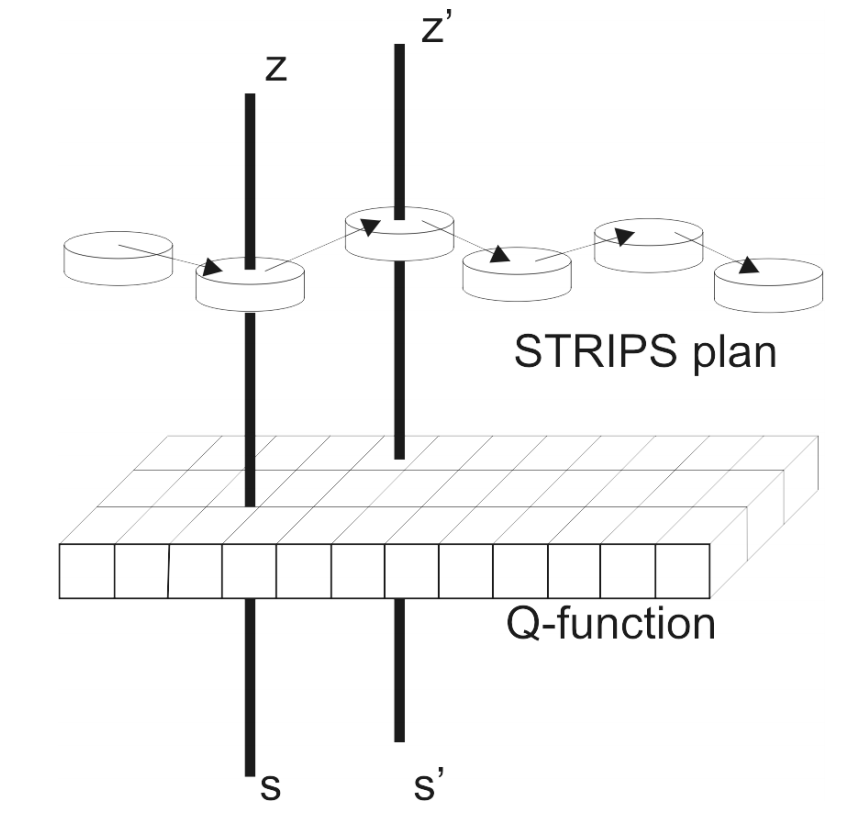
\includegraphics[width=0.75\linewidth]{img/strips.png}
  \caption{Plan-base reward shaping.}
  \label{fig:strips}
\end{figure}


A strips-plan consists in a set of subgoals that the agent should be focusing on in the specified order to increase the total ending reward. These plans are used to encode a potential function that rewards better the agent states that are later in the plan than the states lower in the plan or out of the plan. So that potential function will be used by reward shaping to help the agent's to follow their plan whitout forcing them nor changing their goal. 

\subsubsection{Multi-Agent Planning}
Setting the plans for multi agents can be done in two ways: within one centralised agent or spread amongst several agents.\\
With the centralised agent, it generates a joint plan where agents cooperate with each other but it requires a global view of the problem, i.e sharing information like goals and abilities. Often, this cooperation is not available to the agents.\\
The second approach is to create one plan per agent as it was alone. This way will create conflict plans for the agents.


\subsubsection{Multi-Agent, Plan-Based Reward Shaping}
For both ways of doing, each of these plans are translated into a sequence of states that the agent's states can be compared to. Therefore the agent's potential $\phi$ can be chosen as :\\

$\phi (s) = \omega * CurrentStepInPlan$

$\omega = MaxReward/NumStepsInPlan$\\\\
where $\omega$ is a scaling factor and $CurrentStepInPlan$ is the corresponding plan's step of the agent's state. We will compare the differences between individual and joint plan based reward shaping and we will see the benefits and constraints of each.



\subsection{Study Case}

We choose two agents who starts on the S1 and S2 squares respectively. Their objective is to reach the goal while trying to collect a maximum of flags while doing so. The possible actions here are going up, down, left and right. A state here, is a position in the world space combined with the current step in the plan and the number of flags he collected. At each time step, they will move one square up, down, left or right unless they collide with a wall or the other agent. Each of our agents has to reach the goal to end an episode. When an agent reaches the goal, his episode is over and he will wait the other agent to finish his run before collecting the final reward. In our study case the reward for each state-action pair is always zero unless it leads to the goal where the reward is equal to $100*NumFlagsCollectedTogether$. Also note that we used the $\epsilon -greedy$ algorithm for exploration, but we could use any other exploration algorithm like SoftMax,... The same goes over our choice for SARSA, we could have used any other temporal differance algorithm such as Q-Learning.

\begin{figure}[h!]
\centering
  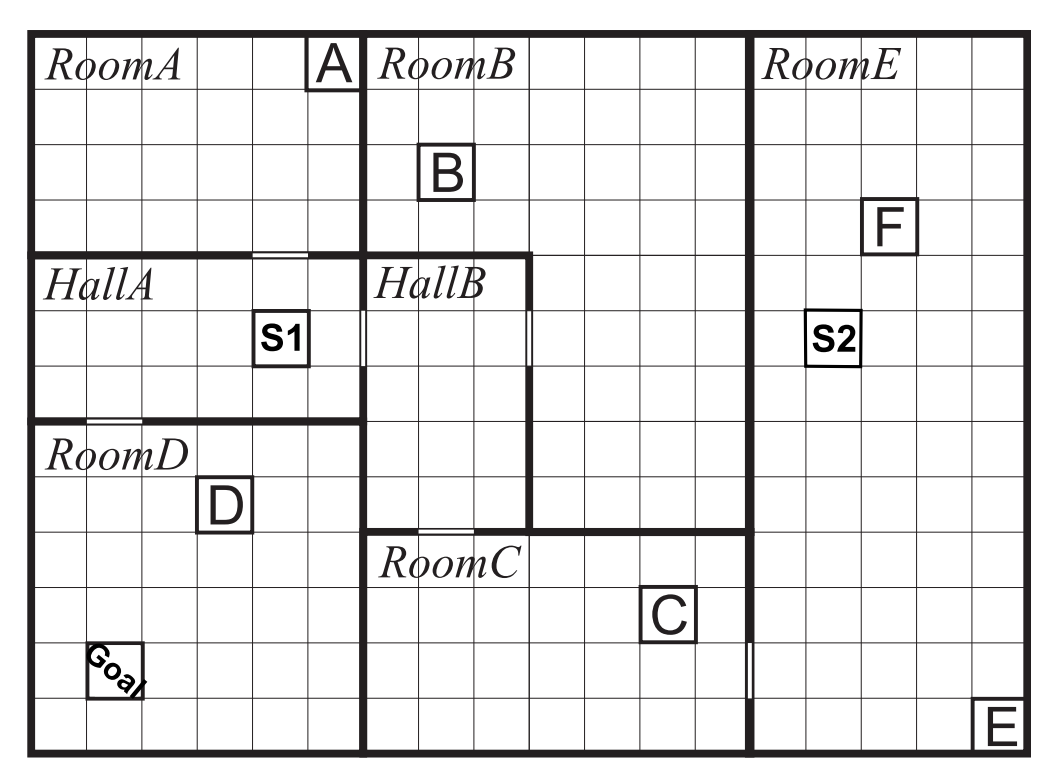
\includegraphics[width=0.75\linewidth]{img/stydyCase.png}
  \caption{Multi-Agent, Flag-Collecting Problem Domain.}
  \label{fig:studycase1}
\end{figure}

\subsubsection{Potential function} 
By adding plans knowledge, we encourage agents to reach some subgoals before reaching the final goal. Our subgoals are : going from a room to another and collecting a flag in the current room when specified. Examples of individual and joint plans we will be using are given on figures \ref{fig:plan1} and \ref{fig:plan2}.

\begin{figure}[h!]
\centering
  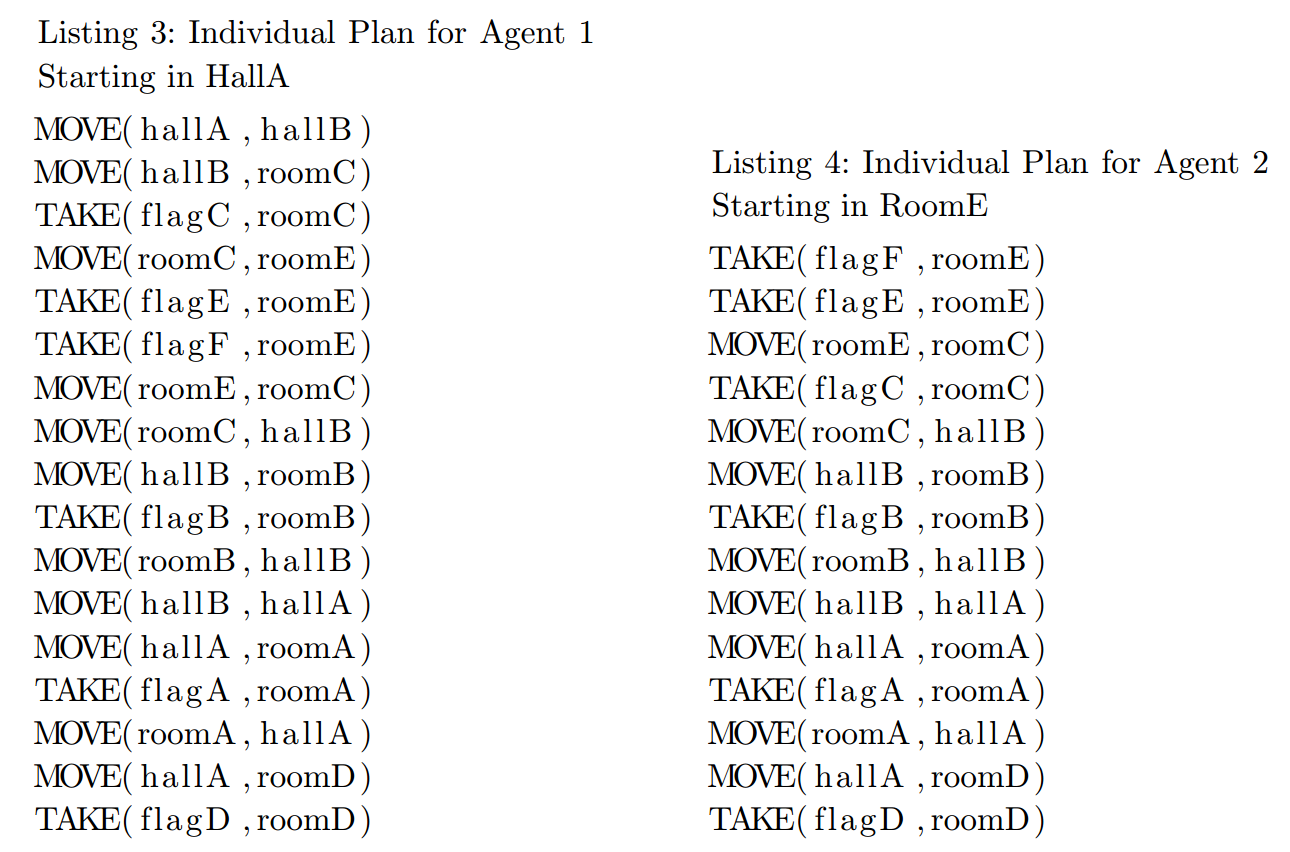
\includegraphics[width=1\linewidth]{img/individualPlan.png}
  \caption{Individual plan.}
  \label{fig:plan1}
\end{figure}

\begin{figure}[h!]
\centering
  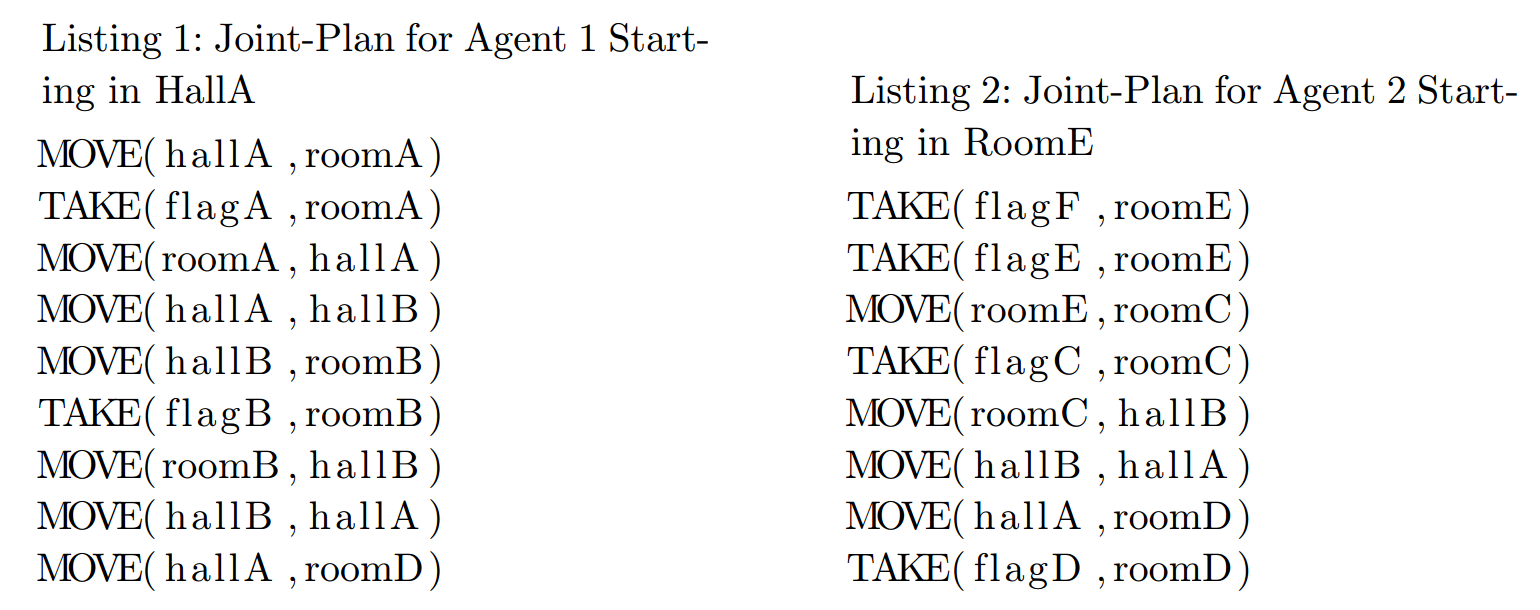
\includegraphics[width=1\linewidth]{img/joinPlan.png}
  \caption{Joint plan.}
  \label{fig:plan2}
\end{figure}

Each of these plans are translated into a sequence of states that the agent should follow as a state-based plan (Figure \ref{fig:plan3}). 

\begin{figure}[h!]
\centering
  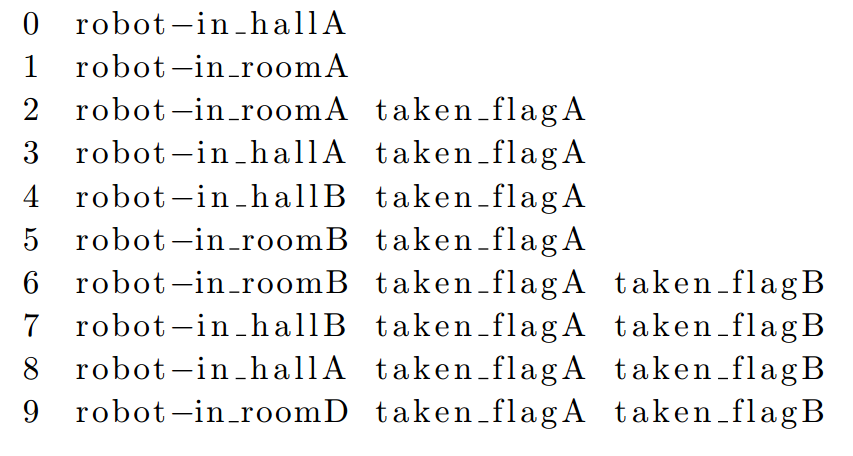
\includegraphics[width=1\linewidth]{img/listingFormattedJoinAgent1.png}
  \caption{State-Based Joint-Plan.}
  \label{fig:plan3}
\end{figure}

The first step in the plan is always true. Then, the agents will move through the world grid and will find themselves either in a further step of the plan or they will deviate from the plan. Based on the plan's step it belongs, one can award it a reward. In case the agents goes into a state that is not stipulated in its plan, it uses the last known step it was in, to avoid defavorising exploration. The previously presented potential function is used.

 We will compare the differences between individual and joint plan based reward shaping and we will see the benefits and constraints of each.\\

We will also compare this heuristic with a flag-based heuristic where the potential function is the number of flags an agent has collected alone times one hundred. \\

$\phi (s) =  NumFlagsCollected*\omega$\\\\
where $\omega = MaxReward/MaxFlagsInWorld$, $NumFlagsInWorld$ is the total number of flags in the world and $NumFlagsCollected$ is the number of flags the agent has collected itself.\\

Finally, those potential functions will be combined into one. When running this new heuristic of flag-based method with individual-plan-based or joint-plan-based shaping, the agent's potential becomes :\\

$\phi (s) = \omega * (CurrentStepInPlan + NumFlagsCollected)$

$\omega = MaxReward/(NumStepsInPlan + NumFlagsInWorld)$\\\\


As one can see, all the potential functions give a maximal reward equivalent to the maximal reward of the goal. It is important to be consistent in this choice in order to set the propention of an agent to follow a policy shaped by reward shaping at a constant level.


\section{Results and Discussion}

For our tests, when ran all experiments 30 times and presented the mean discounter reward per episode in our graphs below. We choose the following values for our parameters : $\lambda$ = 0.4, $\alpha$ = 0.1, $\gamma$ = 0.99, $\epsilon$ = 0.1. Also, all Q-values were initialized to 0.

\subsection{Initial results}

After running thirty times all experiments, the mean discounted reward per episode were plotted on the following graphs. The discounted reward is the goal reward multiplied by the discounted factor exponent the step number needed to reach the goal  \citep{SCpbrs}. This value offers a way to classify the shaping, taking into account the number of flags collected and the time the agents takes to get them.\\
 Our initial case results are shown on Figure \ref{fig:results1}. \\

\begin{figure}[h!]
  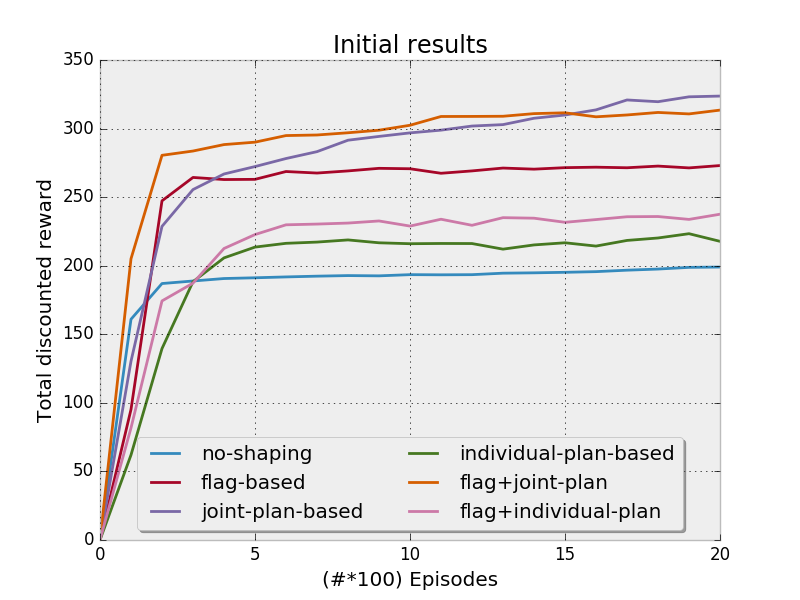
\includegraphics[width=\linewidth]{img/initial.png}
  \caption{Initial results.}
  \label{fig:results1}
\end{figure}

First, it is shown on the results that the learning with no shaping gives the worst outcome. This result was the expected one since knowledge, even poor, improves the behaviour of the agents.\\
Next, as one can see, the joint-plan-based gives the best result. With the joint-plan, the agents cooperates to collect the six flags, i.e the optimal way.\\
About the individual-plan-based shaping, the discounted reward is rather low, just above the no shaping one. This results comes from two main behaviours of the agents with this plan. When analysing the individual plans, one will quickly notice that the agents will jeopardize each other early. Indeed, each agent will try to collect the flag that the other agent needs to collect, they will find themselves in a deadlock situation. The other possible outcome is when agent number two takes all the flags and the other one none as it can be seen on figure \ref{fig:behave}.\\
The flag-based reward shaping get the agents to learn a behaviour where they collect the flags that are on their path leading to a result where the agent goes quickly to the goal but with approximately two third of the flags.\\
When adding the flag-based heuristic to the plan-based one, for the joint-plan it converges quicker but then doesn't give significant differences since the results without it are already optimal. For the individual-plan-based reward shaping, it is clear that adding the flag-based heuristic improves the reward a bit because it adds some knowledge to the agents.\\

\begin{figure}[h!]
  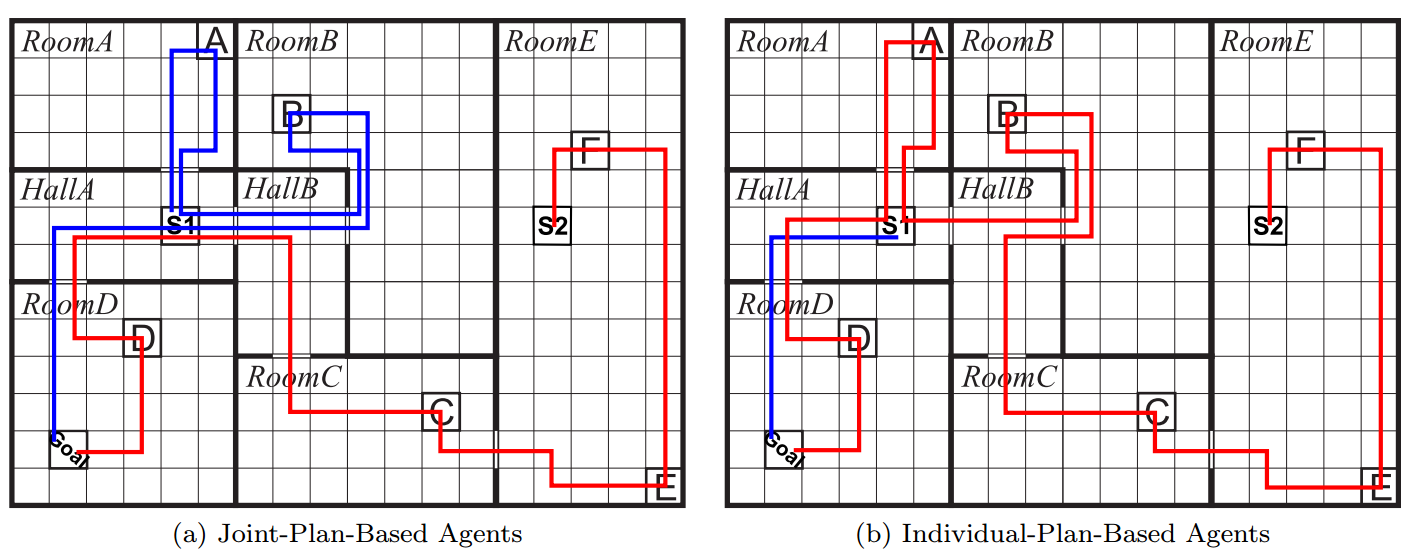
\includegraphics[width=\linewidth]{img/behavious.png}
  \caption{Behaviours of :}
  \label{fig:behave}
\end{figure}

Once those results obtained, our aim was to reduce the gap between the results of the plan based reward shaping with joint plan and individual plan.\\
In order to do so, we explored two methods. The first one is about improving the knowledge of the agents and the second one concern their cooperation.

\subsection{Improved knowledge}

In this section, the main idea is to improve the knowledge of the agents by altering their plan.\\
One should bear in mind that the aim is to tend to the results given by the joint-plan-based rewards shaping since it gives the best output.\\
We saw that one major issue of the individual-plan-based heuristic, is the conflict knowledge. We therefore tried to reduce it.\\
The first way of reducing it was to delay the conflict in the plan to the fifth collected flag whereas it was the fourth flag in the original plan.\\
The other new plans are also individual but they make the agents collect only five or four flags, therefore there are only four or two common flags left.\\
On the graph figure \ref{fig:results2}, the results of those new plans are compared with the no shaping ones and the joint plan based ones. The delayed conflict is represented by plan-based-6 and the two other shaping heuristics represent the one where the individual-plans do not take all the flags.

\begin{figure}[h!]
  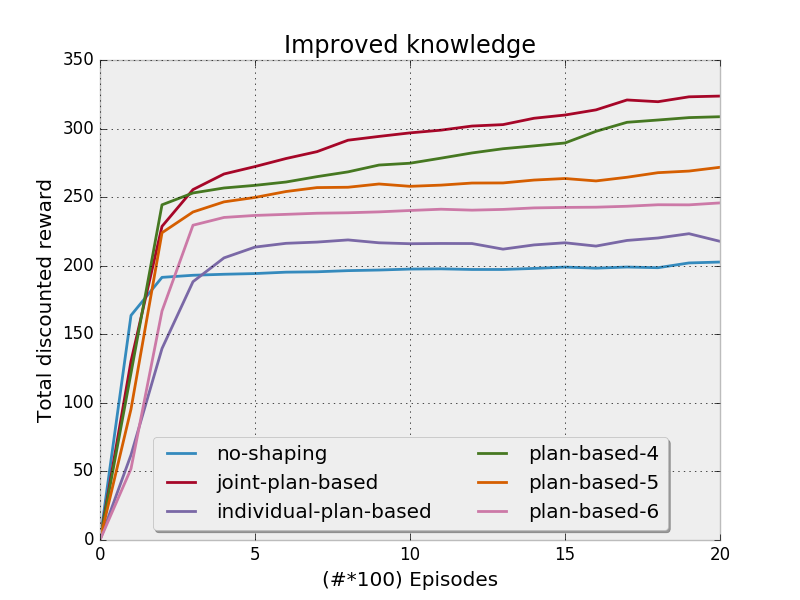
\includegraphics[width=\linewidth]{img/knowledge.png}
  \caption{Improved knowledge.}
  \label{fig:results2}
\end{figure}

As expected, the more delayed the conflict is, the best the results are. Specially, the two outcomes of the individual-plan stayed but when it isn't the one where one agent takes all the flags then the agents collect on average more flags, proportionally to the time before conflicts arise.

\subsection{Improved cooperation}

In this part, the goal was to improve the plan individual-plan-based reward shaping through minimal cooperation between the agents.\\
In this implementation, the agents know if the other agent took a flag. Practically, when one agent collects a flag, he will send a message to the other in order to notice him.\\
Only the original individual plan was tested with this setup. It would not make sense to use it with a joint plan because it will make the agent go in a state that isn't in the plan. The results can be seen in the figure \ref{fig:results3}.

\begin{figure}[h!]
  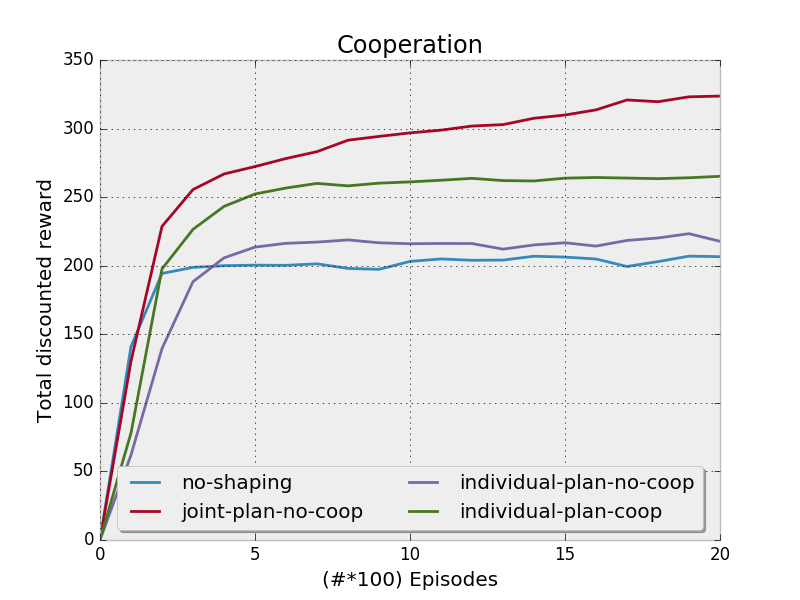
\includegraphics[width=\linewidth]{img/coop.png}
  \caption{Improved cooperation.}
  \label{fig:results3}
\end{figure}

This new cooperation shows a significant improvement in the outcome of the individual plan. It does not reach the joint plan because in this setup the agents will not often collect all flags and they will go for long distances. This behaviour comes from the fact that it was the one intended in the individual plan, here the conflicts are avoided but the plan stay poor.

\section{Conclusion}
In this paper we explored plan-based reward shaping in temporal difference learning with eligibility traces. We compared two types of plans, a joint one and an individual one.\\

Our next goal was to find a way to improve the individual plan in order to reach the results of the joint one.\\
We showed that avoiding conflict knowledge leads to better results. We achieved this by modifying the individual plans. Avoiding enough conflict can almost lead to optimal result.\\
We then added basic cooperation between the agents to overcome those conflicts. The results were better than with no cooperation but there was still a gap between the two plans.\\

Other work suggested that increasing exploration could overcome conflict knowledge as well \citep{paper4}. Another way to avoid conflict goals is to use abstract MDP reward shaping such as it has been proposed \citep{abstractmdp}.

Future work about overcoming conflict knowledge in multi agent learning could be about knowledge revision. It has already be successful for single agent \citep{efthymiadis2014knowledge}. Another think we could think about to change can be comparing different learning algorithms, it would interesting to compare multiagent specifics learning algorithms like General-Sum Games \citep{devlin2013potential}. The last thing that comes to our mind is changing the potential function, perhaps movements off the plan should be punished or skip past plans steps allowed via increased potential despite missing a previous one.




\footnotesize
\bibliographystyle{apalike}
\bibliography{example}


\end{document}
